%\subsection{High throughput binding affinity calculator Workflow}

%\jhanote{Generally not good style to have only 1 subsection in a section and best 
%to eliminate subsection heading}

% BAC uses the Ensemble Toolkit to create a high-throughput workflow which we
% refer to as HTBAC. 

HTBAC is a workflow system that uses RADICAL-Cybertools to implement ESMACS,
and similar protocols such as TIES. These workflows consist of pipelines with
stages comprised of heterogeneous tasks. For example equilibration and
production, followed by post processing steps. 

Although ESMACS and TIES methods are similar at a high-level, viz., they are
comprised of concurrent, multi-stage pipelines with synchronization (Fig.
5(R)), The different protocols supported by HTBAC differ in the details of the
pipelines, stages and synchronization.

HTBAC uses the Ensemble Toolkit (EnTK) API to express these workflows. RADICAL-Cybertools
provides advanced resource management capabilities and, thereby delivers the
necessary high-throughput capabilities required. The framework is generic and
can be simply expanded to run the ESMACS protocol. EnTK provides a common API,
execution and programming model to these different methods, and thus will
minimize development effort and complexity.

The Ensemble Toolkit API exposes four components (‘Resource
Handle’, ‘Pipeline’, ‘Stage’, and ‘Task') to the user which express the
application logic of HTBAC. We describe these components for one of the HTBAC
protocols, ESMACS. The ESMACS protocol contains a set of pipelines where each
pipeline contains functions that operate on a given replica. EnTK interprets these replicas as independent pipelines. Each pipeline consists of multiple stages representing a well-defined execution order; each stage can contina heterogeneous workloads. Although each stage of a pipeline depends on its predecessor, the pipelines execute independent of each other. The pattern within pipelines are identical and describes a set of simulations as shown in Fig~\ref{figure:ESMACS-pipelines}

\begin{figure}[ht]
\centering
  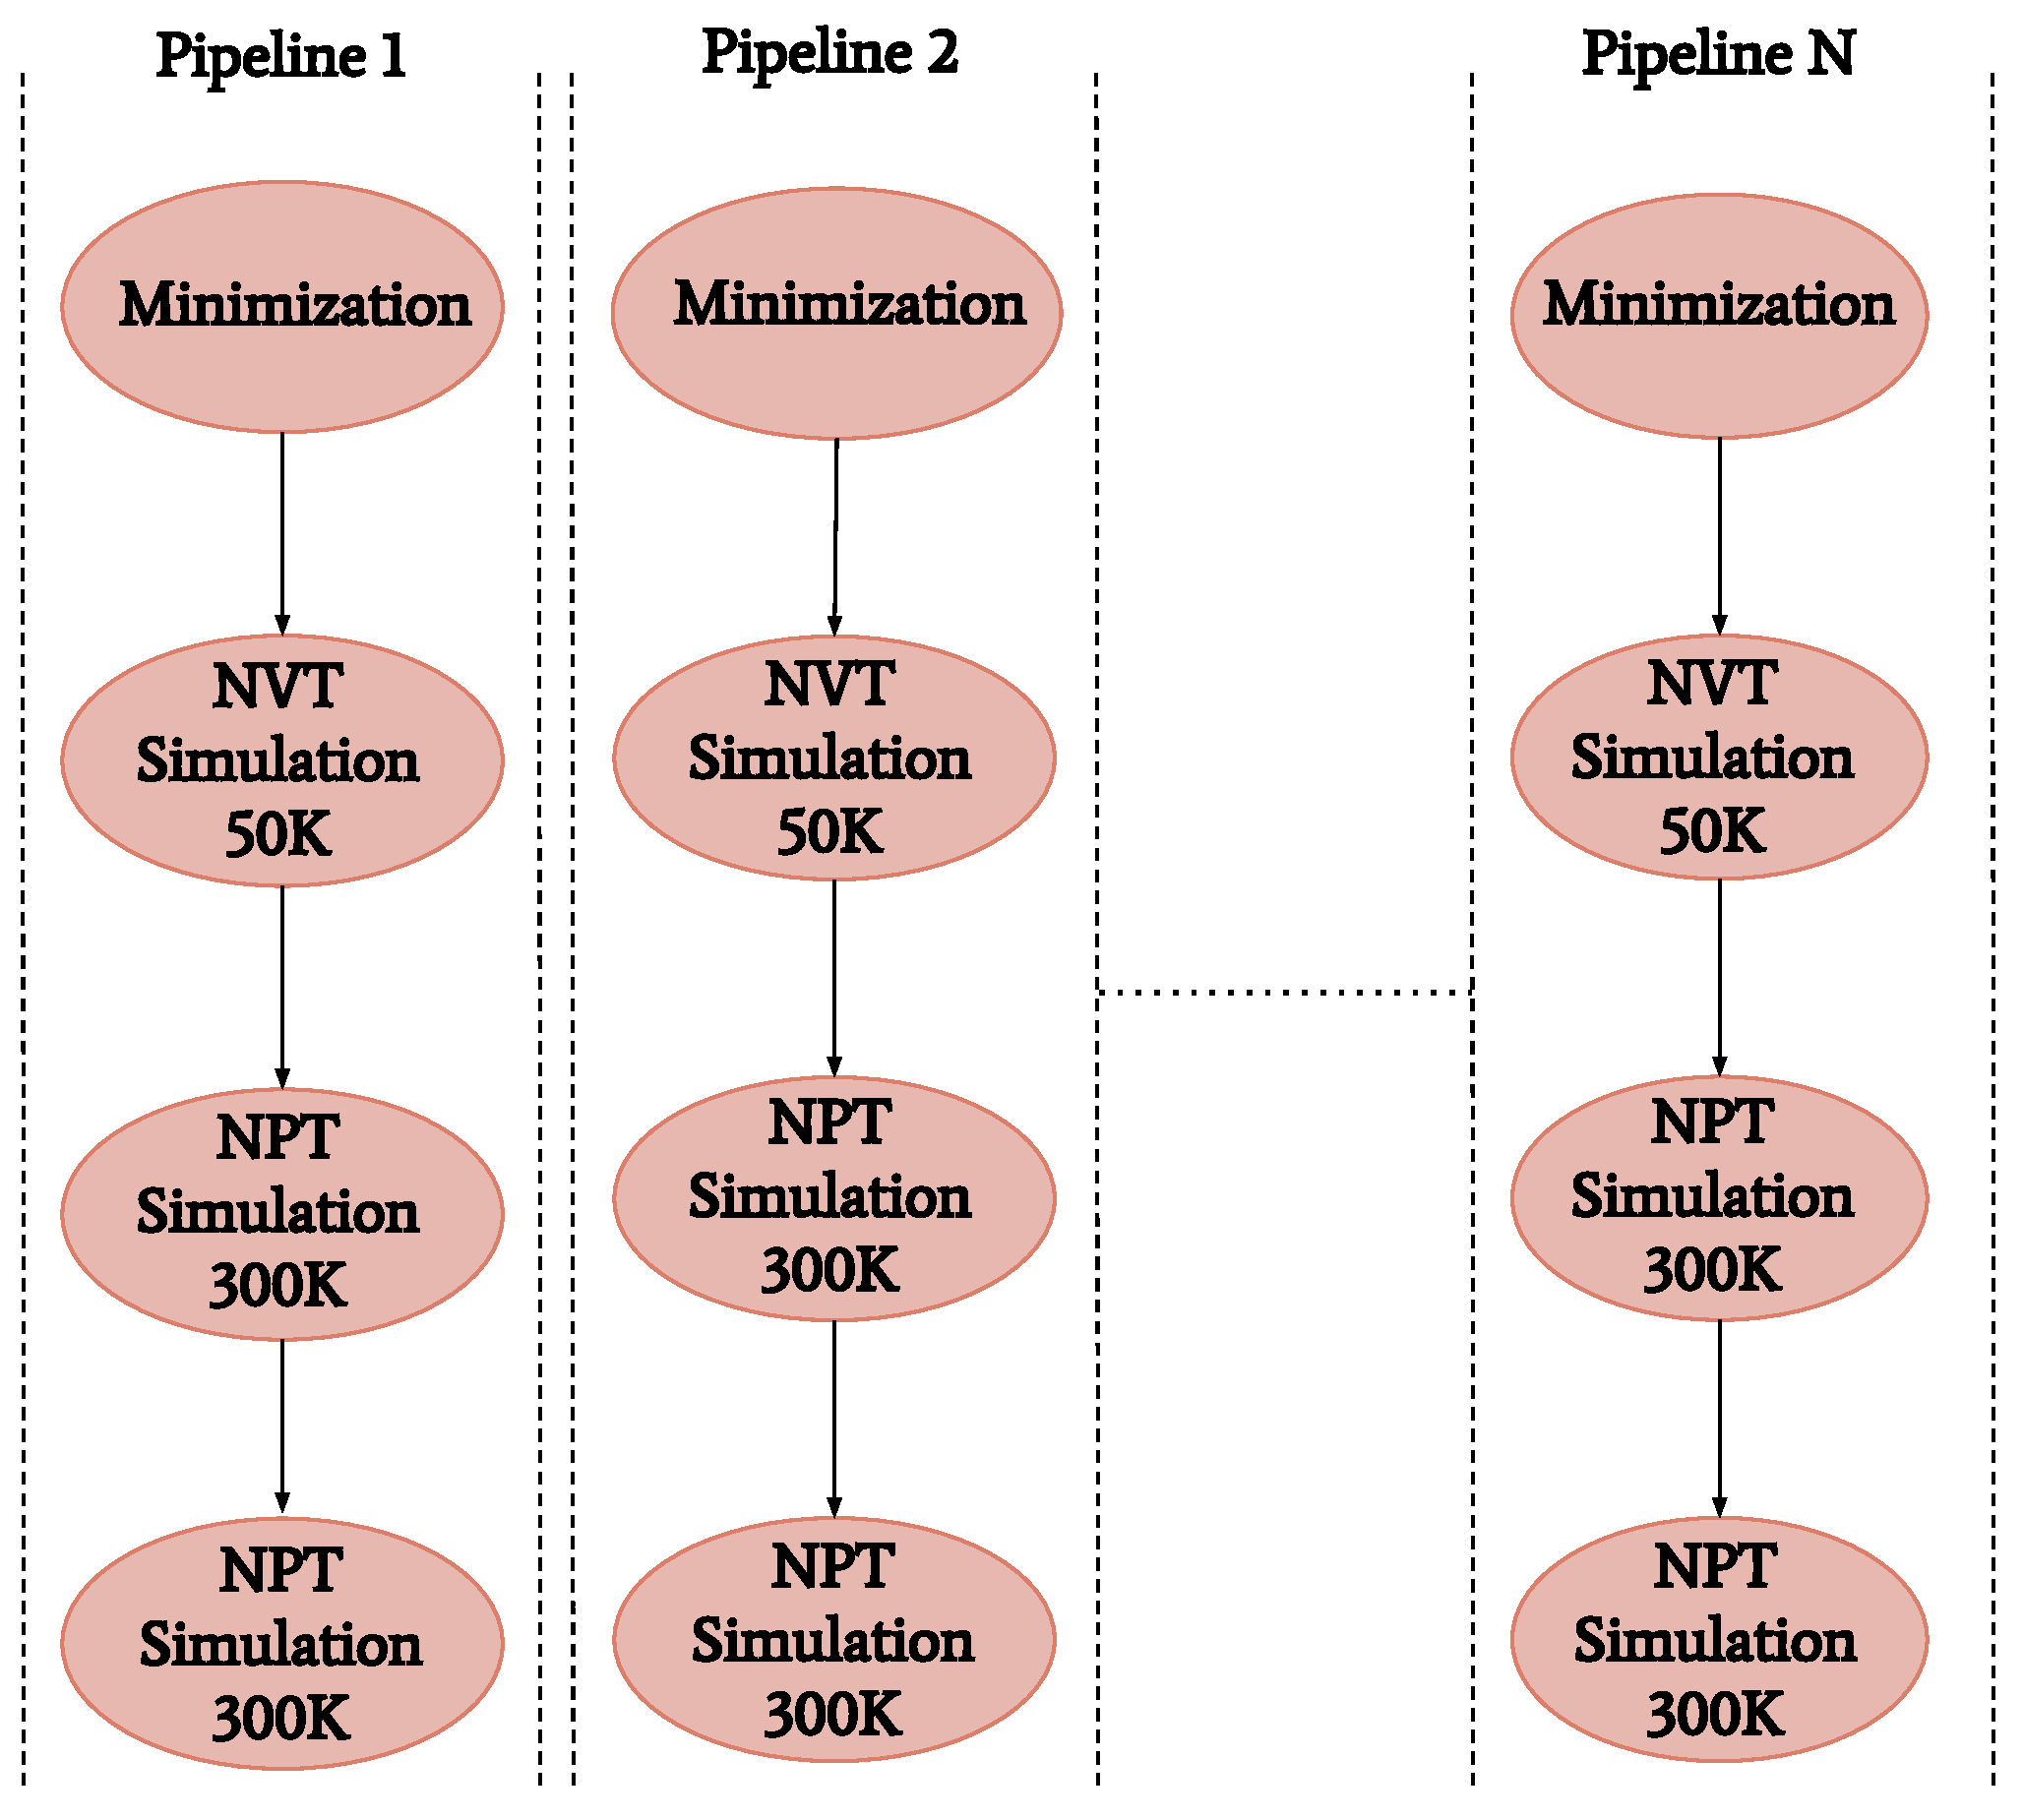
\includegraphics[width=0.5\textwidth]{FIGURES/HT-BAC-NAMD-pipelines-control-flow-only.pdf}
  \caption{\bf ESMACS protocol indicating n-pipelines where each pipeline represents a set of simulations which are captured as stages by EnTK}
   \label{figure:ESMACS-pipelines}
\end{figure}

%\begin{itemize}
%	\item 1) Untar configuration files
%	\item 2) Preprep
%	\item 3) Minimize with decreasing restraints
%	\item 4) Equilibration: NVT simulation at 50K, with restraints
%	\item 5) Equilibration: NPT simulation at 300K, with decreasing restraints 
%	\item 6) Equlibratin: NPT at 300k, no constraints
%	\item 7) Tarball output files 
%\end{itemize}

Each stage is composed of a single unique task which is described by a set of attributes that define the workload parameters such as the location of input files, the number of simulations and the MD engine(s) to launch simulations. The ESMACS protocol defines 7 stages, in which the preliminary and last stages perform staging the input/output data. The middle stages indicate simulation tasks as shown in Fig~\ref{figure:ESMACS-pipelines}. The task is appended to a stage and stages are appended to a pipeline to maintain temporal order. The workflow relies on a resource configuration which consists of the details required to use a resource where the application will be executed including runtime, queue, and account details. We capture the integration of the application (ESMACS protocol) and how it interfaces with EnTK in Fig~\ref{figure:ht-bac_rp}. 

We define the client resource in Fig~\ref{figure:ht-bac_rp} as the workload system-- HTBAC which describes a series of replicas with ordered functions as a pipelines with stages and tasks. EnTK interprets these pipelines as a functional set of tasks and generates the pilot description that contains the resource configuration of how to run the HTBAC workload. For the ESMACS protocol running on Blue Waters we define the runtime system, queue, and the pilot size. Once RADICAL-Pilot receives this new workload it generates a pilot that submits placeholders to the queue. Once the pilot is activated, the RP-Agent submits the tasks in the form of compute units to the placeholders to begin execution.  


\begin{figure}[ht]
\centering
  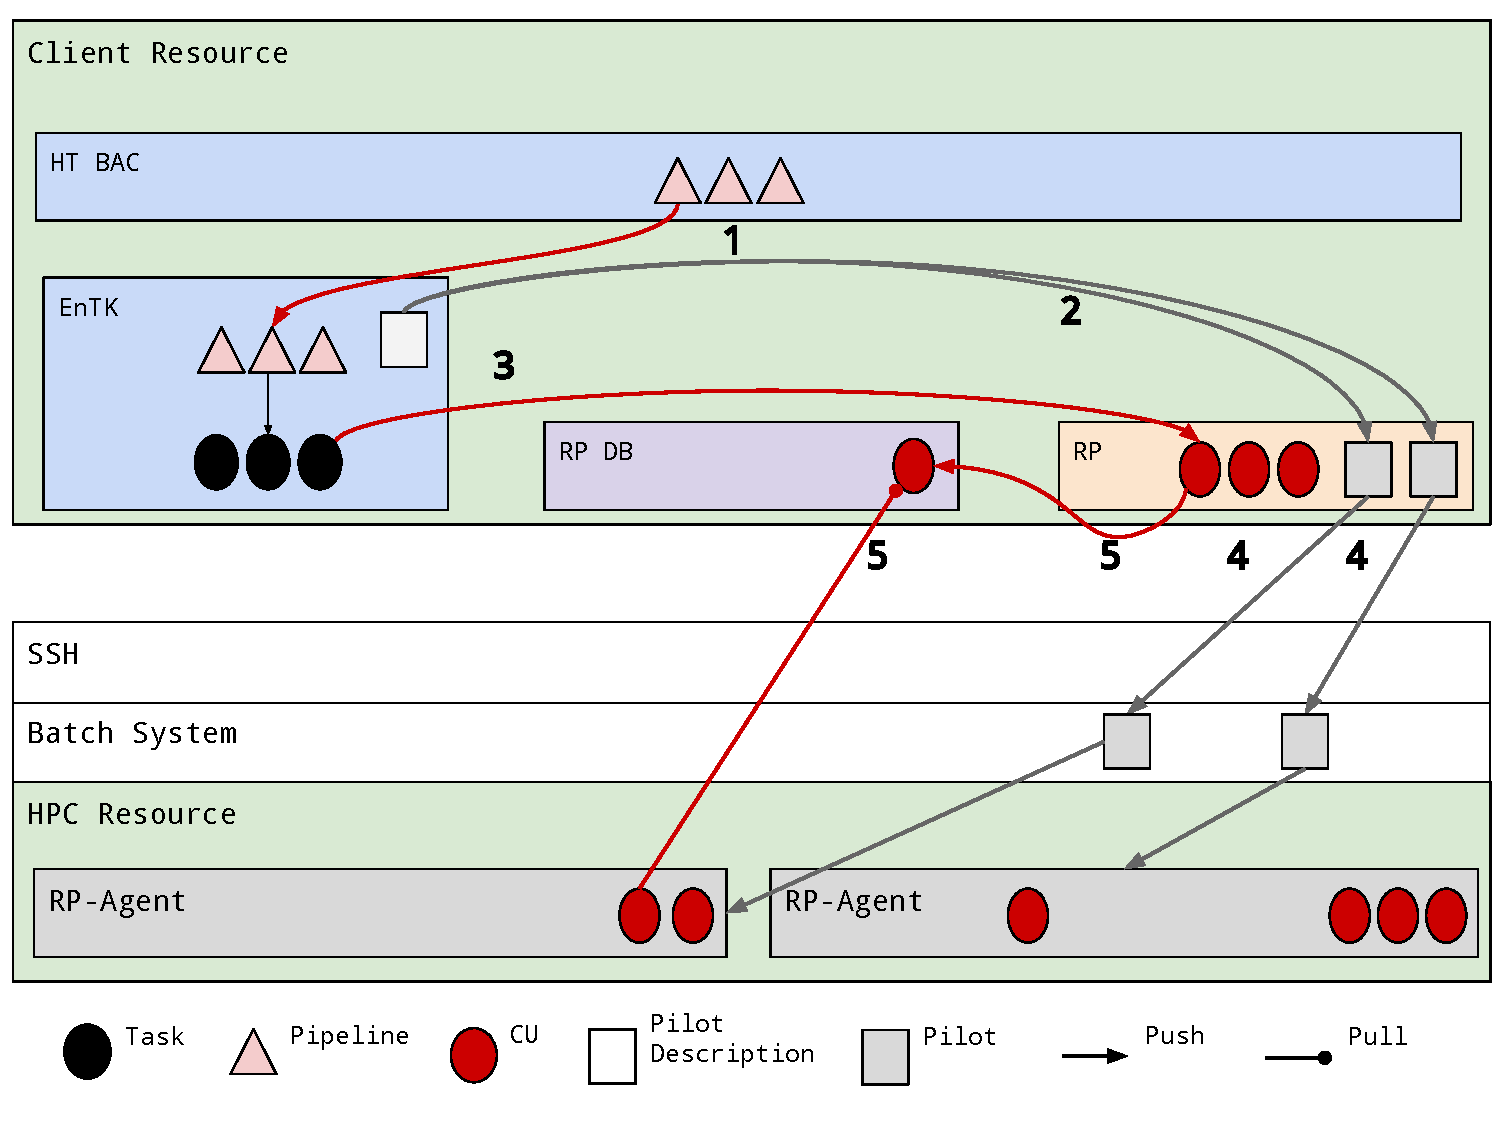
\includegraphics[width=0.5\textwidth]{FIGURES/ht-bac-rp_integration.pdf}
  \caption{\bf Integration between HTBAC workflow and EnTK. Numbers indicate the temporal sequence of execution. RADICAL-Pilot (RP) database (DB) can be deployed on any host reachable from the resources.}
   \label{figure:ht-bac_rp}
\end{figure}

%\begin{figure}[ht]
%\centering
%  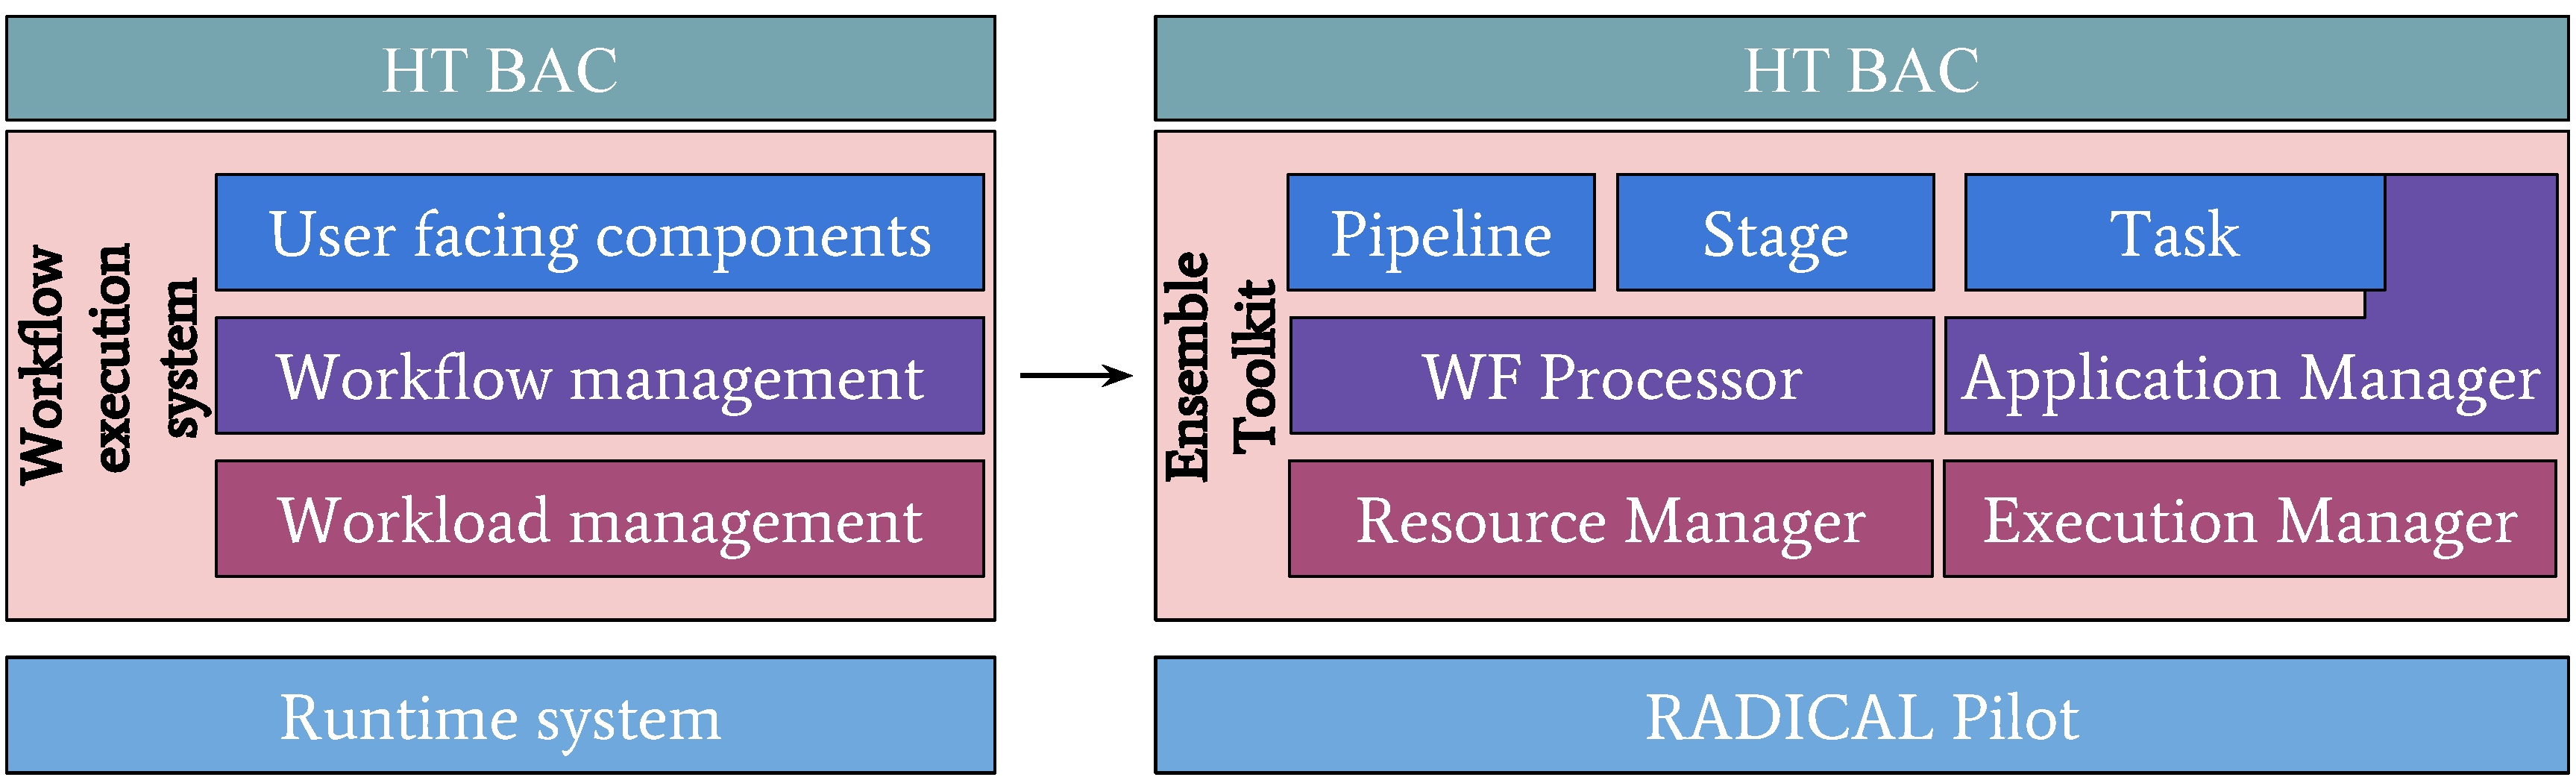
\includegraphics[width=0.5\textwidth]{FIGURES/entk_htbac_integration.pdf}
 % \caption{\bf Integration between HT-BAC workflow system and EnTK that shows resource/application managers.}
   %\label{figure:ht-bac_entk}
%\end{figure}

